\documentclass[11pt,a4paper]{report}

% ta bort numreringen av sections m.m.
%\setcounter{secnumdepth}{-1}
% möjliggör klickbara länkar i innehållsförteckningen
\usepackage{hyperref}
\hypersetup{
  colorlinks,
  citecolor=blue,
  filecolor=blue,
  linkcolor=blue,
  urlcolor=blue
}

% stöd för svenska
\usepackage[swedish]{babel}
% stöd för utf-8
\usepackage[utf8]{inputenc}
% stöd för input, verbatim-block m.m.
\usepackage{verbatim}
% stöd för bilder och att de "flyter" i texten
\usepackage{graphicx}
\usepackage{wrapfig}

% fixa så att kapitel alltid börjar på jämna sidor (höger sida)
\makeatletter
\renewcommand*\cleardoublepage{\clearpage\if@twoside
  \ifodd\c@page \hbox{}\newpage\if@twocolumn\hbox{}%
  \newpage\fi\fi\fi}
\makeatother

% kommandon för framsidan
\title{Tekweb \\ \large{Ett mobilanpassat ramverk för hemsidor}}
\author{Emilio Nyaray      \and
        Filip Gottfridsson \and
        Magnus Söderling   \and
        Markus Säfström
}
\date{\today}

\begin{document}
\maketitle

% begin abstract
\begin{abstract}
Kortfattad sammanfattning av rapporten.
\end{abstract}
% end abstract

\tableofcontents
\newpage

% begin chapter
\chapter{Introduktion}
\section{Bakgrund}
Filips text om projektet.

\section{Mål}
Det vi kom fram till att tekweb skulle klara av under de första mötena.

\section{Begränsningar av projektet}
Här skriver vi vad vi lät bli att göra under arbetet med projektet.
% end chapter

% begin chapter
\chapter{Förarbete}
\section{Brainstorming}
I början av arbetet med projektet så brainstormade projektgruppen för
att få igång det kreativa tänkandet och harmonisera medlemmarnas mål och
visioner kring arbetet med projektet.

\input{brainstorming}

% till mad, om du vill bryta upp det här i två delar så är det bara att
% köra, mönstret för hur man gör det borde gå att utläsa i dokumentet :)
\section{Pappersprototyper och användarintervjuer}
Grejerna mad gjorde när han pappersprototypade och pratade med folk i
foobar.

\input{prototyping_interviews}

% end chapter

% begin chapter
\chapter{Arkitektur}
I detta avsnitt avhandlas ramverket och dess beståndsdelar samt ett
tillägg som gjordes för att möjliggöra förandet av statistik över vilka
sidor som besöks och i viss mån även vilka funktioner som används.

\subsection*{En löst specificerad design}
I början av arbetet med projektet hade vi inte en klar bild av hur
ramverkets arkitektur skulle se ut, men för att påskynda arbetet
implementerades den arkitektur som beskrivs i resten av dokumentet.
Under vårt arbete definierade vi, huvudsakligen genom konventioner, hur
ramverket med dess flexibla grundfunktionalitet skulle användas.

\section{Moduler}
Moduler spelar en central roll i ramverket eftersom de är byggstenarna i
en sida som byggs med Tekweb. En modul är i grunden en klass vars
instans(er) har för syfte att sammanställa och göra information
användbar för en besökare.  Informationen kan läsas in på flera sätt,
Tekweb erbjuder ett simpelt gränssnitt för att läsa ut information från
andra hemsidor som en lång sträng och om behovet finns så kan man även
implementera hjälpklasser för att göra mer avancerad
data-insamling/-manipulering, för att hålla modulklassens komplexitet på
en rimlig nivå.

För att göra modulerna enklare att skriva måste de, enligt konvention,
överskugga någon av metoderna för de olika visningslägena i den
abstrakta klassen ContentModule\footnote{$<$Referens till källkods-filen
som innehåller ContentModule?$>$}. Det ansvar en modul har, ur ett
infrastrukturellt perspektiv är att se till att vissa lokala variabler i
en klassinstans får lämpliga värden som av ramverket sedan utläses för
att generera sidan det ska visas på. Eftersom basklassen och ramverket
sköter transporten av den genererade informationen (XML för internt
bruk) så kan det gå snabbt att skriva en modul, så länge den inte har en
komplicerad uppgift, förstås.

Modulernas innehåll renderas i slutändan på ett av de sätt (om det är
implementerat i modulen) som finns i figur~\ref{list:modes}, beroende på
vilket tillstånd modulen befinner sig i.

\begin{figure}[h]
\begin{itemize}
  \item {\bf Standardläget (default)}  används typiskt för att visa en
    sammanställning av all information som finns tillgänglig för
    användaren.
  \item {\bf Växelläget (toggler)}  används när man vill ha ett
    klickbart objekt på hemsidan som fäller ut en ruta med det önskade
    innehållet när den aktiveras.
  \item {\bf Frestelseläget (teaser)}  används då man vill visa en länk
    som ska fresta användaren till att surfa vidare, t.ex. då man visar
    upp en rubrik till en nyhet.
  \item {\bf AJAX-läget (ajax)}  används för att skapa innehåll som ska
    injiceras i en laddad sida i samverkan med växelläget.
\end{itemize}
\caption{En lista av möjliga tillstånd för moduler\label{list:modes}}
\end{figure}

Eftersom tiden för sidladdning och rendering fortfarande är runt 2-5 (om
inte mer) sekunder på dagens smartphones så ville vi minimera antalet
sidladdningar. För att åstadkomma detta införde vi växelläget, så som
det beskrivs i figur~\ref{list:modes}.

\subsection{Standardläget}
Standardläget är det tillstånd en modul kommer att befinna sig i om
inget annat anges i konfigurationsfilen. I detta tillstånd kommer
modulen att generera sitt innehåll som renderas på det sättet
standardlägets visningsmall definierar.

\subsection{Växelläget}
Växelläget fungerar i två steg; $1$) modulen genererar ett
aktiveringsobjekt, d.v.s. något klickbart som användaren ser (möjligen
en bild som ser ut som en app-ikon), $2$) om/när modulens
aktiveringsobjekt aktiveras av användaren kommer innehållet att hämtas
och injiceras i platsen där modulen renderats på sidan.

Eftersom innehållet hämtas med javascript är det möjligt att användaren
deaktiverat javascript eller har en undermålig javascriptimplementation
som inte klarar av att göra ajax-förfrågningar. Om man behöver hantera
alla besökare, oavsett om de har javascript eller ej, kan man göra så
att datagenereringen i ajax-läget och standardläget sker på samma sätt.
Det blir då möjligt att låta växelläget generera ett aktiveringsobjekt
som är en länk till en sidvisning med den aktuella modulen i sitt
standardläge. Om användaren kan hantera javascript så slipper den en
tidsödslande sidladdning, om inte så tar det lite längre tid, men
fungerar fortfarande. Termen för detta är \dq graceful degradation\dq.

\subsection{Frestelseläget}
Frestelseläget används för att locka användare till att klicka på länkar
för att få se något innehåll, det kan t.ex. vara en rubrik från en
nyhet, inledningen på ett twittermeddelande o.s.v.

\subsection{Ajaxläget}
Ajaxläget används, i ramverket, inte ensamt utan endast i samverkan med
växelläget (se ovan).

\subsection{Hjälpfiler}
Utöver den PHP-fil som modulenklassen är implementerad i så används i
vissa fall även någon/några av följande hjälpfiler;

\begin{itemize}
  \item PHP-fil(er) med hjälpklasser.
  \item JavaScript-fil(er) som innehåller funktionalitet som behövs hos
    klienten.
  \item XSL-mall(ar) som bestämmer hur modulens generererade XML-kod ska
    transformeras till HTML.
  \item CSS-fil(er) som används för att definiera hur den genererade
    HTML-koden ska presenteras för användaren.
\end{itemize}

\section{Konfigurationsfilen}
Ramverket konfigureras med en XML-fil som är uppbyggd enligt
figur~\ref{fig:xml-config}.

\begin{figure}[h]
\begin{verbatim}
                         root
                 _________|_______...__
                 |     |     |        |
               title  item  item     item
                       |     |        |
                       .     .        .
                       .     .        .
                       .     .        .
\end{verbatim}
\caption{Illustration av konfigurationsfilen}
\label{fig:xml-config}
\end{figure}

Rot-noden ({\it root}) innehåller alltså en titel-nod ({\it title}) och
ett godtyckligt antal modul-noder ({\it item}). I {\it title} finns en
sträng som senare används för att sätta sidans titel.

{\it item} används för att beskriva de modul-instanser som ska finnas på
sidan och hur de ska vara konfigurerade. Noden kapslar in {\it module},
{\it mode} och {\it settings} som anger vilken modul det är som ska
instansieras, vilket visningsläge instansen kommer att köras i
respektive inställningar som behövs för att modulen ska fungera
och/eller kunna göra mer.

\section{Mallsystemet}
Eftersom vi tidigt insåg att vi skulle behöva någon typ av mallsystem så
valde vi att använda oss av XSLT-mallar. Valet motiverades med att
verktygen som skulle behövas för att konvertera mallarna redan fanns på
plats på webb-hotellet och dessutom var standardiserade, två väldigt
starka argument då man arbetar med webben. XSLT-mallar används alltså
för att det innehåll som genereras av modulerna ska kunna presenteras på
ett sätt som slutanvändarens webbläsare kan hantera.

För att vi snabbt skulle kunna få ut innehåll från flera moduler
bestämde vi att modulerna skulle generera XML på en viss form för att
minska mallskrivandet överlag.

XSLT-mallarna används ibland även internt, för att transformera
aggregerad information. Schemamodulen använder sig av
XSLT-transformationer för att transformera inläst kalenderdata från ett
datorvänligt format till ett mobilvänligt format, mer om detta i
modulens avsnitt.

\section{Ramverket}
\marginpar{\footnotesize Skriv något om inbyggda funktioner här?}

Den centrala delen av ramverket, som sköter genereringen av innehållet,
ligger i $htdocs/index.php$ och är i grunden uppbyggd av tre steg:

\begin{itemize}
  \item {\bf Förberedelsen}
    I detta steg förbereds PHP-miljön för att kunna exekvera modulerna
    genom att;

    \begin{itemize}
      \item $a)$ länka in nödvändig funktionalitet som finns definierad
        i andra filer,
      \item $b)$ eventuellt trimma den laddade konfigurationen,
      \item $c)$ ladda konfigurationen och
      \item $d)$ ladda huvudsidans mall,
    \end{itemize}

    för att kunna generera huvudsidan.

    I vissa fall kan förfrågan som för tillfället besvaras vara endera
    en AJAX-fråga eller en förfrågan om att få en viss undersida. I
    dessa fall kommer det att göras en kontroll för att avgöra huruvida
    det är en giltig förfrågan. Om frågan visar sig vara giltig så
    kommer den laddade konfigurationen att anpassas därefter i steg $b$
    ovan.

  \item {\bf Huvud-loopen}
    Huvud-loopen.

  \item {\bf Utskriften}
    I detta steg skrivs det genererade innehållet helt enkelt ut.
\end{itemize}

\section{Användargränssnitt}
\label{sec:ui}
Här skriver vi mer om hur vi tänkte med UI:et och varför det är
ssssmmmmexxayyy!

\section{Utbyggnader}
\label{design:stats}
Här skriver Magnus några rader om hur han haxX0rade in statistik-fixen.

% end chapter

% begin chapter
\chapter{Implementation}
I detta kapitel beskrivs implementationen av den arkitektur som beskrevs
i det föregående kapitlet.

\section{Ramverket}
Ramverket är skrivet i PHP och förlitar sig på följande
moduler/bibliotek;

\begin{itemize}
  \item[{\bf Output Buffering}] Utskrifter som vanligen hade gått till
    klientens webbläsare går istället till en buffert för mellanlagring.

  \item[{\bf Session}] Används för att lagra sessionsspecifik data.

  \item[{\bf DOM}] För att arbeta med konfigurationsfilen och intern data.

  \item[{\bf XSL}] För att transformera data som läses ut från andra tjänster
    på internet och i universitetets nät.
\end{itemize}

\subsection{Filträd}
Tekwebs filer lagras enligt följande struktur;

\begin{verbatim}
 /
|- conf/
| |- config.php
| |- root.xml
| |- root.xsl
|- css/
| |- layout.css
| |- module/
| | |- <modulspecifika css-filer>
| |- reset.css
| |- style.css
|- gfx/
| |- <instansspecifika bilder>
| |- icons/
| | |- <modulikoner>
| |- module/
|   |- <modulkataloger>
|- htdocs/
| |- index.php
|- include/
| |- <modulers hjälpbibliotek>
| |- contentmodule.php
| |- core.php
|- index.php
|- js/
| |- <modulers javascript-filer> 
| |- main.js
|- module/
| |- <modulkataloger>
|   |- <modul>.php
|   |- [<xsl-mall>.xsl]
|- tekweb.tmproj
\end{verbatim}


\section{Modulerna}
De moduler som i dagsläget finns implementerade är;

\begin{itemize}
  \item {\bf about} används för att visa en ``om''-text, d.v.s. en kort
    text om hemsidan;

  \item {\bf empsearch} låter användaren söka efter personer på en
    LDAP-server;

  \item {\bf feed} läser ut RSS-flöden (även andra sorter((????))) och
    presenterar dem på ett trevligt sätt;

  \item {\bf multifeed} kombinerar \emph{feed}-instanser för att
    aggregera innehåll från olika källor till ett uniformt flöde;

  \item {\bf statictext} presenterar statiskt innehåll för användaren;

  \item {\bf timeedit} ligger som ett lager ovanpå det befintliga
    TimeEdit-systemet och gör ett mobilvänligt användargränssnitt.

  \item {\bf uumap} visar busshållsplatser, nationshus, m.m. Filip får
    skriva här, han gjorde maaaassoooor!

\end{itemize}

%\input{about}
%\input{empsearch}
%\input{feed}
%\input{multifeed}
%\input{statictext}
%\subsection{Timeedit}
I det följande avsnittet kommer TekNat-fakultetens instans av
planeringsverktyget Timeedit att kallas för tjänsten. Den modul i tekweb
vid namn timeedit som arbetar mot tjänsten kommer att kallas för
modulen.

\subsubsection{Bakgrund}
Text som beskriver bakgrunden till modulen

\subsubsection{Mål}
Modulens syfte är att tillgängliggöra den funktionalitet som är synlig
mot studenterna hos tjänsten. Modulen skapades eftersom projektgruppen
och beställaren tidigt var överens om att de tänkta användarna skulle
betrakta funktionaliteten som en kärnfunktion.

\subsubsection{Begränsningar}
Här skriver vi om de medvetna begränsningar som gjordes av modulen
p.g.a. tidsbegränsningar, svåra tekniska problem, buggar, m.m.

\subsubsection{Informationsflöde}
Att beskriva modulen i sitt sammanhang samt den hjälpklass som används
(LibTimeEdit) görs bäst genom att först visa informationsflödet med
hjälp av följande bild och sedan sätta ord kring det som visas i bilden
nedan.

Beskriv saker som modulen gör, relatera dem till bilden.

\begin{wrapfigure}{r}{0.5\textwidth}
  \begin{center}
    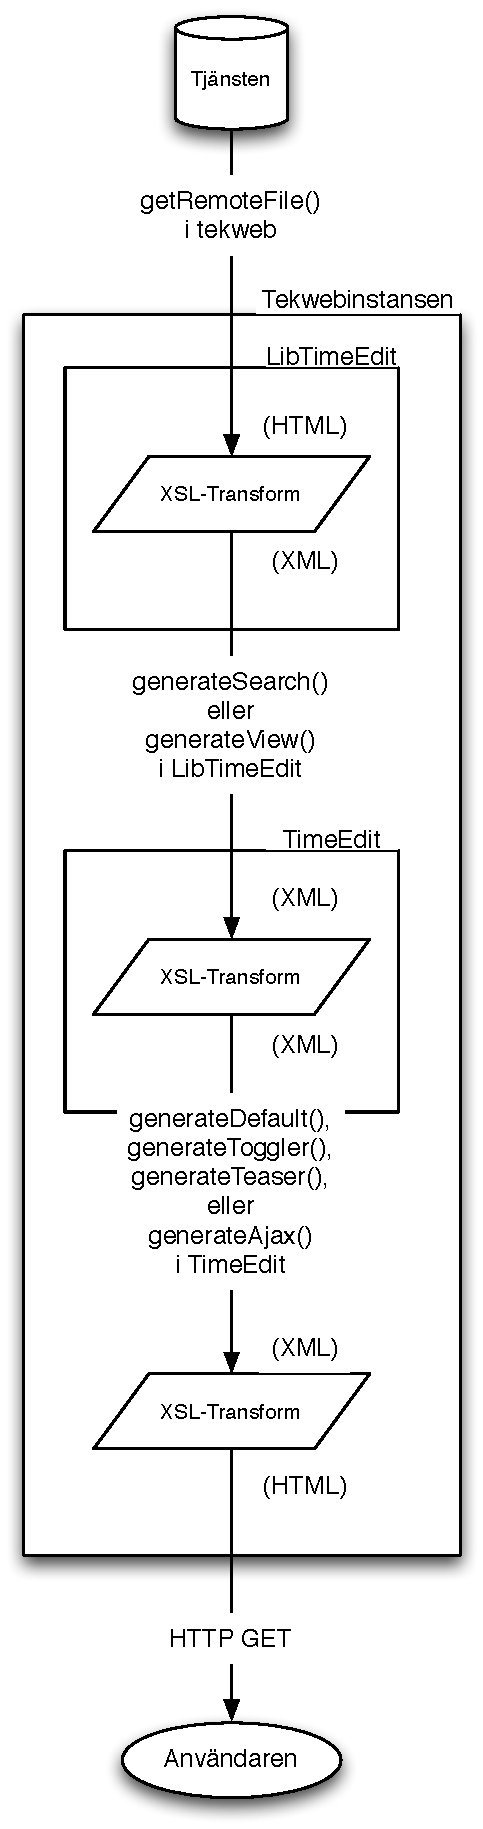
\includegraphics[width=45mm]{timeeditchart.pdf}
  \end{center}
  \caption{TimeEdit i sitt sammanhang.}
\end{wrapfigure}


%\input{uumap}



% end chapter

% begin chapter
\chapter{Utvärdering}
Hur gick det att genomföra projektet? Var det något särskilt som gick
bra/dåligt?

\input{evaluation}

% end chapter

% begin chapter
\chapter{Slutsatser}
Vi lyckades bygga en funktionell prototyp som tillgängliggjorde den
funktionalitet och information som på förhand bestämts med beställaren.

\input{conclusions}

% end chapter

% begin chapter
\chapter{Fortsatt arbete}
Skriva om vissa saker, bygga ut andra, rätta till knasigheter.

% bilagor...

\end{document}

